\NeedsTeXFormat{LaTeX2e}
%\PassOptionsToClass{handout}{beamer}
\documentclass{beamer}
\usepackage{beamerPack}
\usepackage[boxed,ruled,vlined]{algorithm2e}
\usepackage{setspace}
\usepackage[usestackEOL]{stackengine}[2013-10-15]
\def\x{\hspace{4.1ex}}    %BETWEEN TWO 1-DIGIT NUMBERS
\def\y{\hspace{3.4ex}}  %BETWEEN 1 AND 2 DIGIT NUMBERS
\def\z{\hspace{2.7ex}}    %BETWEEN TWO 2-DIGIT NUMBERS
\usepackage[04]{../lecture}
\subtitle{練習問題}
\begin{document}

\begin{frame}[fragile]{}
\titlepage
\end{frame}

\section{algorithm design}		%%%%%%%%
\subsection{}

\begin{frame}[fragile]{問題解決の枠組み}{}
\begin{enumerate}%\itemsep8pt
\item 問題の解法をアルゴリズム化する\footnotemark
\begin{align*}
アルゴリズム = & 前処理? 相似問題^{+} 後処理?
\end{align*}
\item (要求を満たすまでオーダーレベルの無駄を省く)
\item 実装する
\item (要求を満たすまで高速化する)
\end{enumerate}

\vfill

\begin{codeof}{language=Rust}{skeleton}
fn solve(problem) {
  ...   // pre process
  solve(sub_problem1);
  ...
  solve(sub_problemN);
  ...    // post process
}
\end{codeof}

\footnotetext[1]{記号はBNFより輸入}
\end{frame}

\begin{frame}[fragile]{アルゴリズムでは再帰であること}{}
fact(100), Fib(100), A(3, 3)を求めるプログラムを作成せよ
\begin{align*}
fact(1) =& 1 \\
fact(n) =& n \times fact(n - 1)\\
Fib(1) =& 1 \\
Fib(2) =& 1 \\
Fib(n) =& Fib(n - 1) + Fib(n -2) \\
A(0, n) =& n + 1 \\
A(m, 0) =& A(m - 1, 1) \\
A(m, n) =& A(m - 1, A(m, n - 1))
\end{align*}

\begin{itemize}%\itemsep8pt
\item $T(n) = ? + T(-) + ?$ :: 線形再帰
\item $T(n) = ? + T(-)$ :: 線形再帰、特に末尾再帰
\item $T(n) = ? + T(-) + T(-) + ?$ :: 線形再帰でない
\end{itemize}
\end{frame}

\section{A series of practices}		%%%%%%%%
\subsection{}

\begin{frame}[fragile]{問題0}{}
\stackMath
\Longstack[l]{
n=0\\
n=1\\
n=2\\
n=3\\
n=4\\
n=5\\
n=6\\
n=7\qquad\ \\
}
\Longstack{
1\\
1\x 1\\
1\x 2\x 1\\
1\x 3\x 3\x 1\\
1\x 4\x 6\x 4\x 1\\
1\x 5\y 10\z 10\y 5\x 1\\
1\x 6\y 15\z 20\z 15\y 6\x 1\\
1\x 7\x 21\z 35\z 35\z 21\y 7\x 1\\
}

$n = 23$, 左から11番目の数は?
\end{frame}

\begin{frame}[fragile]{Pascalの三角形}{北東+北西に等しい}
\begin{align*}
P(n,k) &= P(n-1, k - 1) + P(n - 1, k)
\end{align*}

\begin{center}
\rotatebox{-45}{
\scalebox{0.6}{
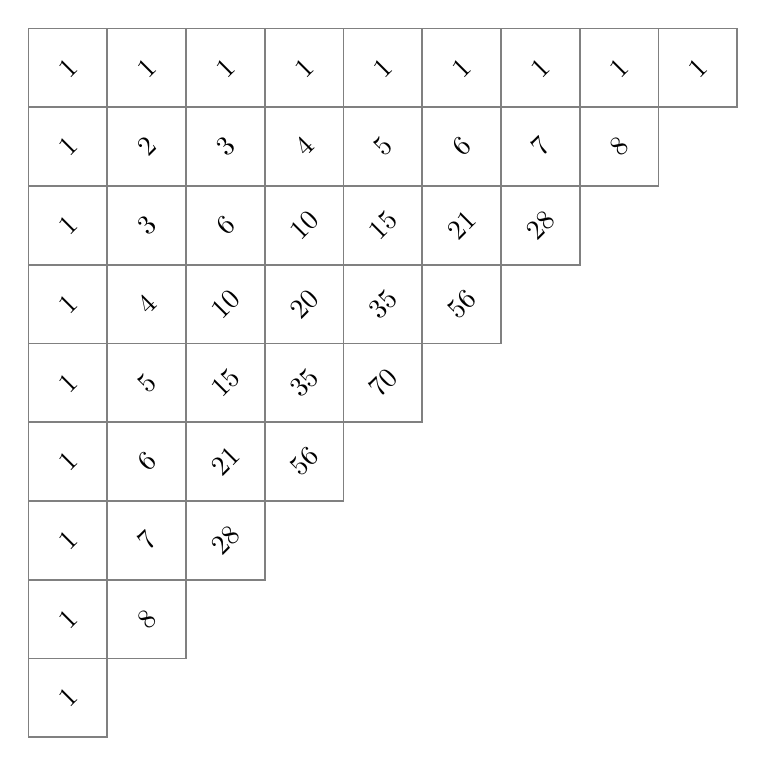
\begin{tikzpicture}[cell/.style = {rectangle,draw=gray,semithick,minimum size=1cm,outer sep=0mm}]
\foreach \i [count=\j from 0] in {1, 1, 1, 1, 1,  1, 1, 1, 1}
    \node[cell] at (\j,  0) {\rotatebox{45}{$\i$}};
\foreach \i [count=\j from 0] in {1, 2, 3, 4, 5,  6, 7, 8}
    \node[cell] at (\j, -1) {\rotatebox{45}{$\i$}};
\foreach \i [count=\j from 0] in {1, 3, 6, 10,15,21,28}
    \node[cell] at (\j, -2) {\rotatebox{45}{$\i$}};
\foreach \i [count=\j from 0] in {1, 4, 10,20,35,56}
    \node[cell] at (\j, -3) {\rotatebox{45}{$\i$}};
\foreach \i [count=\j from 0] in {1, 5, 15,35,70}
    \node[cell] at (\j, -4) {\rotatebox{45}{$\i$}};
\foreach \i [count=\j from 0] in {1, 6, 21,56}
    \node[cell] at (\j, -5) {\rotatebox{45}{$\i$}};
\foreach \i [count=\j from 0] in {1, 7, 28}
    \node[cell] at (\j, -6) {\rotatebox{45}{$\i$}};
\foreach \i [count=\j from 0] in {1, 8}
    \node[cell] at (\j, -7) {\rotatebox{45}{$\i$}};
\foreach \i [count=\j from 0] in {1}
    \node[cell] at (\j, -8) {\rotatebox{45}{$\i$}};
\end{tikzpicture}
}
}
\end{center}
\end{frame}

\begin{frame}[fragile]{イメージしやすい形に回転}{}
\begin{center}
\scalebox{0.5}{
\begin{tikzpicture}[cell/.style = {rectangle,draw=gray,semithick,minimum size=1cm,outer sep=0mm}]
\foreach \i [count=\j from 0] in {1, 1, 1, 1, 1,  1, 1, 1, 1}
    \node[cell] at (\j, 0) {\rotatebox{0}{$\i$}};
\foreach \i [count=\j from 0] in {1, 2, 3, 4, 5,  6, 7, 8}
    \node[cell] at (\j, 1) {\rotatebox{0}{$\i$}};
\foreach \i [count=\j from 0] in {1, 3, 6, 10,15,21,28}
    \node[cell] at (\j, 2) {\rotatebox{0}{$\i$}};
\foreach \i [count=\j from 0] in {1, 4, 10,20,35,56}
    \node[cell] at (\j, 3) {\rotatebox{0}{$\i$}};
\foreach \i [count=\j from 0] in {1, 5, 15,35,70}
    \node[cell] at (\j, 4) {\rotatebox{0}{$\i$}};
\foreach \i [count=\j from 0] in {1, 6, 21,56}
    \node[cell] at (\j, 5) {\rotatebox{0}{$\i$}};
\foreach \i [count=\j from 0] in {1, 7, 28}
    \node[cell] at (\j, 6) {\rotatebox{0}{$\i$}};
\foreach \i [count=\j from 0] in {1, 8}
    \node[cell] at (\j, 7) {\rotatebox{0}{$\i$}};
\foreach \i [count=\j from 0] in {1}
    \node[cell] at (\j, 8) {\rotatebox{0}{$\i$}};
\draw[arrow] (0, -1) -- ++(10, 0) node[below] {N=23 (X=23)};
\draw[arrow] (-1, 0) -- ++(0, 10) node[left] {Y};
\draw[arrow] (10, 0) -- ++ (-6, 6) node[right=5pt, anchor=west] {左から11};
\end{tikzpicture}
}
\end{center}
求める場所は座標$(12, 11)$に対応
\end{frame}

\begin{frame}[fragile]{配列の是非}{}

与えられた問題は点(12, 11)を求める

これは大きさ(12,12)の表を完成させる問題を解けば簡単に求められる

\begin{center}
\scalebox{0.6}{
\begin{tikzpicture}[node distance=5cm, auto]
\node (P) {(12, 11)計算問題};
\node (E) [right of=P] {全点計算問題};
\node (A1) [below of=P] {アルゴリズム1};
\node (A2) [below of=E] {プログラム2};
\draw[->,dashed] (P) to node {なぜ?} (E);
\draw[->] (P) to node {再帰} (A1);
\draw[->] (E) to node {for文 $\times$ for文} (A2);
\draw[->] (A2) to node[below=20pt] {無駄を省くため考え直し} (A1);
\end{tikzpicture}
}
\end{center}
「配列を使ってはいけません」という追加制約があっても解けるのならOK
\end{frame}

\begin{frame}[fragile]{問題1.0}{}
\begin{tikzpicture}[overlay, xshift=0.5\textwidth,yshift=-0.2\textheight]
\node at (0,0) {\pgfimage[width=1.0\pagewidth]{shuttle.jpg}};
\end{tikzpicture}
\textcolor{white}{
観光用スペースシャトルが高度100キロメートルからツアーを開始します。乗客は1分ごとに次の1分間上昇するか、下降するかを決めることができます。どちらも1分でちょうど1キロ上昇するか下降します。61分後(60回の進路変更)に元の高度に戻ってこなければならないとすると、飛行経路は何通りあるでしょう。
}
\end{frame}

\begin{frame}[fragile]{}{}
\begin{center}
\rotatebox{45}{
\scalebox{0.4}{
\begin{tikzpicture}[cell/.style = {rectangle,draw=gray,semithick,minimum size=1cm,outer sep=0mm}]
\foreach \i [count=\j from 0] in {1, 1, 1, 1, 1,  1, 1, 1, 1}
    \node[cell] at (\j,  0) {\rotatebox{-45}{$\i$}};
\foreach \i [count=\j from 0] in {1, 2, 3, 4, 5,  6, 7, 8}
    \node[cell] at (\j, -1) {\rotatebox{-45}{$\i$}};
\foreach \i [count=\j from 0] in {1, 3, 6, 10,15,21,28}
    \node[cell] at (\j, -2) {\rotatebox{-45}{$\i$}};
\foreach \i [count=\j from 0] in {1, 4, 10,20,35,56}
    \node[cell] at (\j, -3) {\rotatebox{-45}{$\i$}};
\foreach \i [count=\j from 0] in {1, 5, 15,35,70}
    \node[cell] at (\j, -4) {\rotatebox{-45}{$\i$}};
\foreach \i [count=\j from 0] in {1, 6, 21,56}
    \node[cell] at (\j, -5) {\rotatebox{45}{$\i$}};
\foreach \i [count=\j from 0] in {1, 7, 28}
    \node[cell] at (\j, -6) {\rotatebox{-45}{$\i$}};
\foreach \i [count=\j from 0] in {1, 8}
    \node[cell] at (\j, -7) {\rotatebox{-45}{$\i$}};
\foreach \i [count=\j from 0] in {1}
    \node[cell] at (\j, -8) {\rotatebox{-45}{$\i$}};
\node at (10,-10) {\rotatebox{-45}{\textcolor{red}{ゴール}}};
\end{tikzpicture}
}
}
\end{center}
60で元の高さ $\to$ 座標(?,?)
\end{frame}

\begin{frame}[fragile]{問題1.1}{}
観光用飛行機が高度5キロメートルからツアーを開始します。乗客は1分ごとに次の1分間上昇するか、下降するかを決めることができます。どちらも1分でちょうど1キロ上昇するか下降します。61分後(60回の進路変更後)に元の高度に戻ってこなければならないとすると、飛行経路は何通りあるでしょう。高度0キロメートルで墜落します。
\end{frame}

\begin{frame}[fragile]{}{}
\begin{center}
\rotatebox{45}{
\scalebox{0.5}{
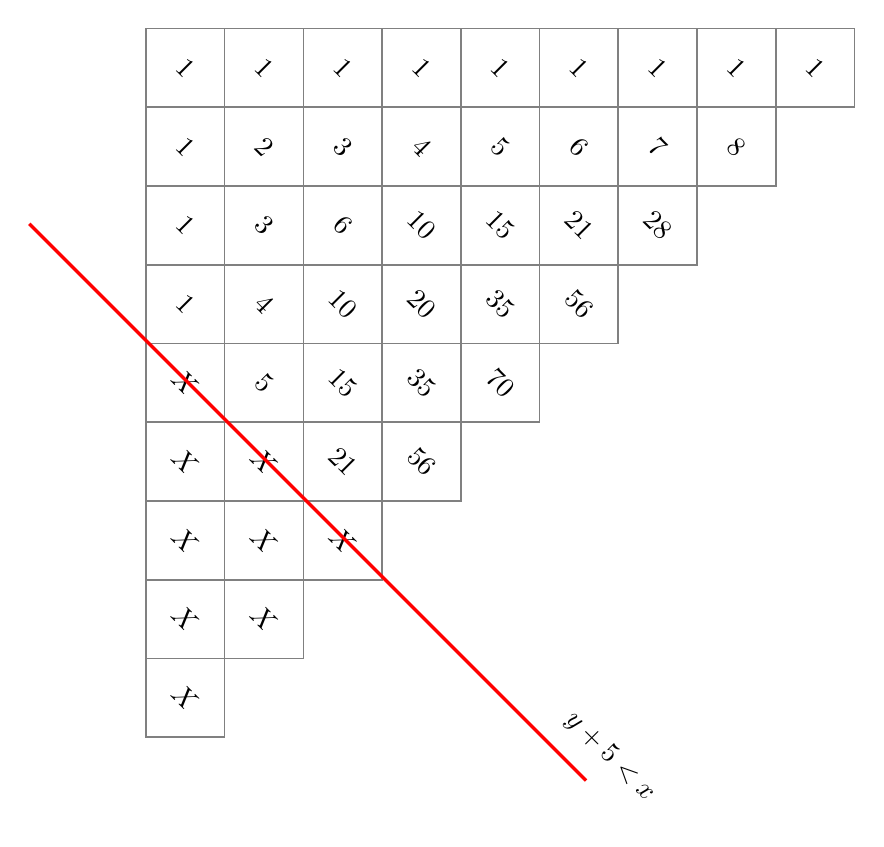
\begin{tikzpicture}[cell/.style = {rectangle,draw=gray,semithick,minimum size=1cm,outer sep=0mm}]
\foreach \i [count=\j from 0] in {1, 1, 1, 1, 1, 1, 1, 1, 1}
    \node[cell] at (\j,  0) {\rotatebox{-45}{$\i$}};
\foreach \i [count=\j from 0] in {1, 2, 3, 4, 5,  6, 7, 8}
    \node[cell] at (\j, -1) {\rotatebox{-45}{$\i$}};
\foreach \i [count=\j from 0] in {1, 3, 6, 10,15,21,28}
    \node[cell] at (\j, -2) {\rotatebox{-45}{$\i$}};
\foreach \i [count=\j from 0] in {1, 4, 10,20,35,56}
    \node[cell] at (\j, -3) {\rotatebox{-45}{$\i$}};
\foreach \i [count=\j from 0] in {X, 5, 15, 35, 70}
    \node[cell] at (\j, -4) {\rotatebox{-45}{$\i$}};
\foreach \i [count=\j from 0] in {X, X, 21, 56}
    \node[cell] at (\j, -5) {\rotatebox{-45}{$\i$}};
\foreach \i [count=\j from 0] in {X, X, X}
    \node[cell] at (\j, -6) {\rotatebox{-45}{$\i$}};
\foreach \i [count=\j from 0] in {X, X}
    \node[cell] at (\j, -7) {\rotatebox{-45}{$\i$}};
\foreach \i [count=\j from 0] in {X}
    \node[cell] at (\j, -8) {\rotatebox{-45}{$\i$}};
\draw[draw=red,rotate=-45,very thick] (0,-2.8) --  ++(10,0) node[rotate=-45,above=4pt] () {$y + 5 < x$};
\end{tikzpicture}
}
}
\end{center}
\end{frame}

\begin{frame}[fragile]{問題2.0}{}
あなたはA地点でお客を拾ったタクシードライバーです。お客はB地点に行こうとしています。
リアルタイム混雑情報サービスはそれぞれのブロック間の移動時間を以下のように表示しています(無限大は工事中)。
最短で何分あればお客をB地点に届けることができるでしょう。
ただしどの道も一方通行です。

\begin{center}
\scalebox{0.5}{
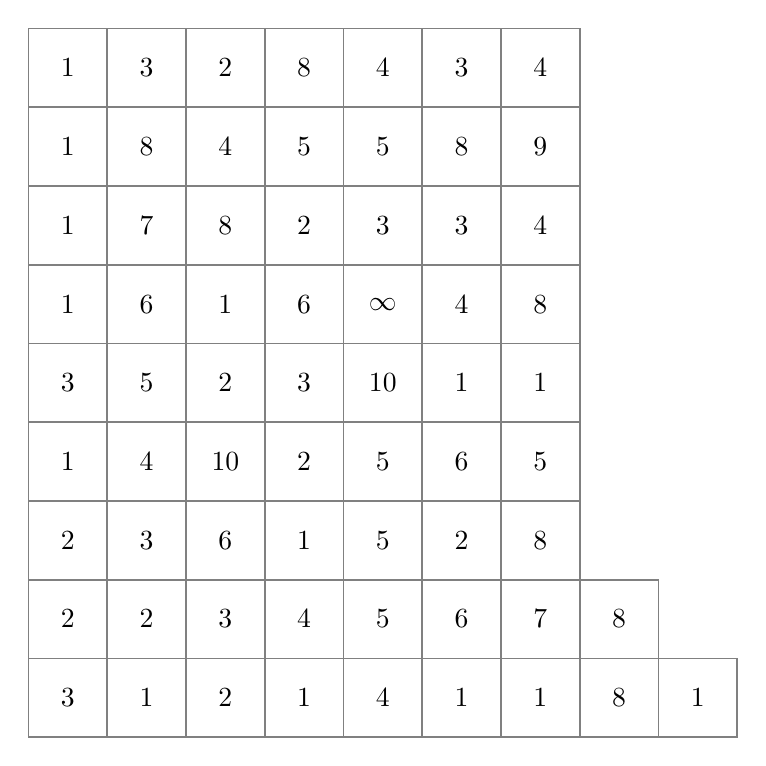
\begin{tikzpicture}[cell/.style = {rectangle,draw=gray,semithick,minimum size=1cm,outer sep=0mm}]
\foreach \i [count=\j from 0] in {3, 1, 2, 1, 4,  1, 1, 8, 1}
    \node[cell] at (\j, 0) {\rotatebox{0}{$\i$}};
\foreach \i [count=\j from 0] in {2, 2, 3, 4, 5,  6, 7, 8}
    \node[cell] at (\j, 1) {\rotatebox{0}{$\i$}};
\foreach \i [count=\j from 0] in {2, 3, 6, 1,5,2, 8}
    \node[cell] at (\j, 2) {\rotatebox{0}{$\i$}};
\foreach \i [count=\j from 0] in {1, 4, 10,2,5 ,6, 5}
    \node[cell] at (\j, 3) {\rotatebox{0}{$\i$}};
\foreach \i [count=\j from 0] in {3, 5, 2,3, 10, 1, 1}
    \node[cell] at (\j, 4) {\rotatebox{0}{$\i$}};
\foreach \i [count=\j from 0] in {1, 6, 1, 6, \infty, 4, 8}
    \node[cell] at (\j, 5) {\rotatebox{0}{$\i$}};
\foreach \i [count=\j from 0] in {1, 7, 8, 2, 3, 3, 4}
    \node[cell] at (\j, 6) {\rotatebox{0}{$\i$}};
\foreach \i [count=\j from 0] in {1, 8, 4, 5, 5, 8, 9}
    \node[cell] at (\j, 7) {\rotatebox{0}{$\i$}};
\foreach \i [count=\j from 0] in {1, 3, 2, 8, 4, 3, 4}
    \node[cell] at (\j, 8) {\rotatebox{0}{$\i$}};
\end{tikzpicture}
}
\end{center}
\end{frame}

\begin{frame}[fragile]{問題2.1}{}
あなたはA地点でお客を拾ったタクシードライバーです。お客はB地点に行こうとしています。
リアルタイム混雑情報サービスはそれぞれのブロック間の移動時間を以下のように表示しています(無限大は工事中)。
最短で何分あればお客をB地点に届けることができるでしょう。

\begin{center}
\scalebox{0.5}{
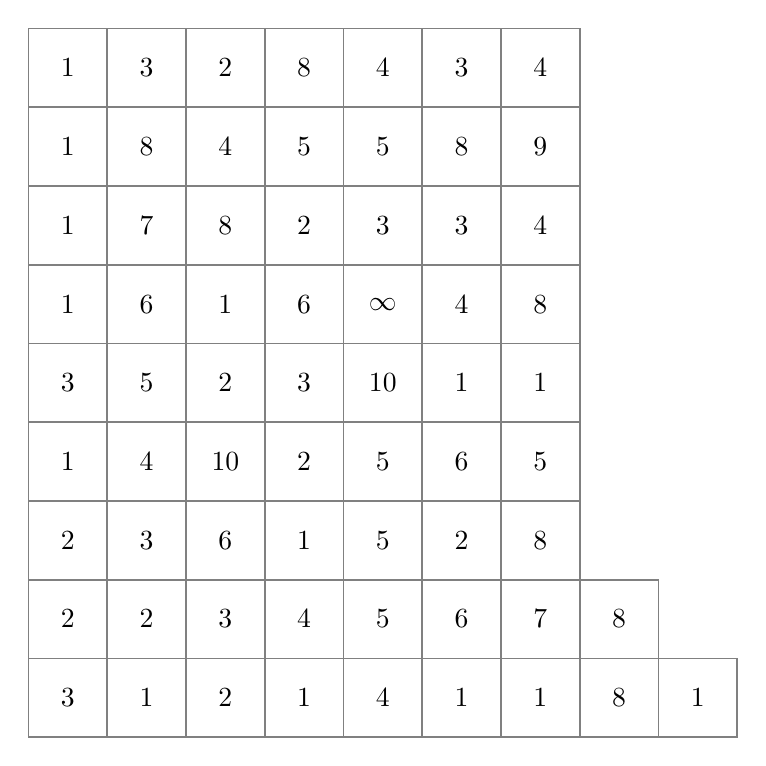
\begin{tikzpicture}[cell/.style = {rectangle,draw=gray,semithick,minimum size=1cm,outer sep=0mm}]
\foreach \i [count=\j from 0] in {3, 1, 2, 1, 4,  1, 1, 8, 1}
    \node[cell] at (\j, 0) {\rotatebox{0}{$\i$}};
\foreach \i [count=\j from 0] in {2, 2, 3, 4, 5,  6, 7, 8}
    \node[cell] at (\j, 1) {\rotatebox{0}{$\i$}};
\foreach \i [count=\j from 0] in {2, 3, 6, 1,5,2, 8}
    \node[cell] at (\j, 2) {\rotatebox{0}{$\i$}};
\foreach \i [count=\j from 0] in {1, 4, 10,2,5 ,6, 5}
    \node[cell] at (\j, 3) {\rotatebox{0}{$\i$}};
\foreach \i [count=\j from 0] in {3, 5, 2,3, 10, 1, 1}
    \node[cell] at (\j, 4) {\rotatebox{0}{$\i$}};
\foreach \i [count=\j from 0] in {1, 6, 1, 6, \infty, 4, 8}
    \node[cell] at (\j, 5) {\rotatebox{0}{$\i$}};
\foreach \i [count=\j from 0] in {1, 7, 8, 2, 3, 3, 4}
    \node[cell] at (\j, 6) {\rotatebox{0}{$\i$}};
\foreach \i [count=\j from 0] in {1, 8, 4, 5, 5, 8, 9}
    \node[cell] at (\j, 7) {\rotatebox{0}{$\i$}};
\foreach \i [count=\j from 0] in {1, 3, 2, 8, 4, 3, 4}
    \node[cell] at (\j, 8) {\rotatebox{0}{$\i$}};
\end{tikzpicture}
}
\end{center}
\end{frame}

\end{document}
